% intro/intro.tex

\chapter{Introduction}
\label{chp:Introduction}

\QuickQuizChapter{chp:Introduction}

Why is parallel programming hard?
One could list any number of reasons, ranging from deadlocks to race conditions
to testing coverage, but the real answer is that {\em it is not really
all that hard}.
After all, if parallel programming was really so horribly difficult,
how could a large number of open-source projects, ranging from Apache
to MySQL to the Linux kernel, have managed to master it?

A better question might be: ''Why is parallel programming {\em perceived}
to be so difficult?''
To see the answer, let's go back to the year 1991.
Paul McKenney was walking across the parking lot to Sequent's benchmarking
center carrying six dual-80486 Sequent Symmetry CPU boards, when he suddenly
realized that he was carrying several times the price of the house he had
just purchased.\footnote{
	Yes, this sudden realization {\em did} cause him to walk quite
	a bit more carefully.
	Why do you ask?}
This high cost of parallel systems meant that
parallel programming was restricted to a privileged few who
worked for an employer who either manufactured or could afford to
purchase machines costing upwards of \$100,000 --- in 1991 dollars US.

In contrast, in 2006, Paul finds himself typing these words on a
dual-core x86 laptop.
Unlike the dual-80486 CPU boards, this laptop also contains 2GB of
main memory, a 60GB disk drive, a display, Ethernet, USB ports, wireless,
and Bluetooth.
And the laptop is more than an order of magnitude cheaper than
even one of those dual-80486 CPU boards, even before taking inflation
into account.

Parallel systems have truly arrived.
They are no longer the sole domain of a privileged few, but something
available to almost everyone.

The earlier restricted availability of parallel hardware
is the \emph{real} reason that parallel programming is considered so difficult.
After all, it is quite difficult to learn to program even the simplest
machine if you have no access to it.
Since the age of rare and expensive parallel machines is for the most
part behind us, the age during which
parallel programming is perceived to be mind-crushingly difficult is
coming to a close.\footnote{
	Parallel programming is in some ways more difficult than sequential
	programming, for example, parallel validation is more difficult.
	But no longer mind-crushingly difficult.}

The purpose of this book is to help you understand how to program
shared-memory parallel machines without risking your sanity.\footnote{
	Or, perhaps more accurately, without much greater risk to your
	sanity than that incurred by non-parallel programming.
	Which, come to think of it, might not be saying all that much.
	Either way, Appendix~\ref{cha:app:Important Questions} discusses
	some important questions whose answers are less intuitive in
	parallel programs than they are in sequential program.}
By describing the algorithms and designs that have worked well in
the past, we hope to help you avoid at least some of the pitfalls
that have beset parallel projects.
But you should think of this book as a foundation on which to build,
rather than as a completed cathedral.
You mission, if you choose to accept, is to help make further progress
in the exciting field of parallel programming, progress that should
in time render this book obsolete.

However, even though parallel programming might not be as hard as
is commonly advertised, it is often more work than sequential
programming.

\QuickQuiz{How could parallel programming \emph{ever} be as easy
	   as sequential programming???}
\QuickQuizAnswer{
	   It depends on the programming environment.
	   SQL~\cite{DIS9075SQL92} is an underappreciated success
	   story, as it permits programmers who know nothing about parallelism
	   to keep a large parallel system productively busy.
	   We can expect more variations on this theme as parallel
	   computers continue to become cheaper and more readily available.
	   For example, one possible contender in the scientific and
	   technical computing arena is Matlab*p @@@ cite @@@,
	   which is an attempt to automatically parallelize comon
	   matrix operations.
} \QuickQuizEnd

It therefore makes sense to consider alternatives to parallel programming.
However, it is not possible to reasonably consider alternativee without
understanding your goals.

\section{Parallel Programming Goals}
\label{sec:intro:Parallel Programming Goals}

@@@ Rewrite based on HOTPAR submission when published. @@@

What should your goals be when programming parallel systems?
Clearly, completing a correctly running program is always job 1.

But if performance is not a concern, you should instead do yourself
a favor and just write single-threaded code.
It will be easier, and you will probably get done much more quickly.

However, Moore's Law has ceased to provide its traditional performance
benefits, as can be seen in
Figure~\ref{fig:intro:Clock-Frequency Trend for Intel CPUs}.
This means that writing single-threaded code and simply waiting
a years or two for the CPUs to catch up may no longer be an option.
Given the recent trends on the part of all major manufacturers towards
multicore/multithreaded systems, parallelism is the way to go for
those wanting the avail themselves of the full performance of their
systems.

\begin{figure}[htb]
\begin{center}
\resizebox{3in}{!}{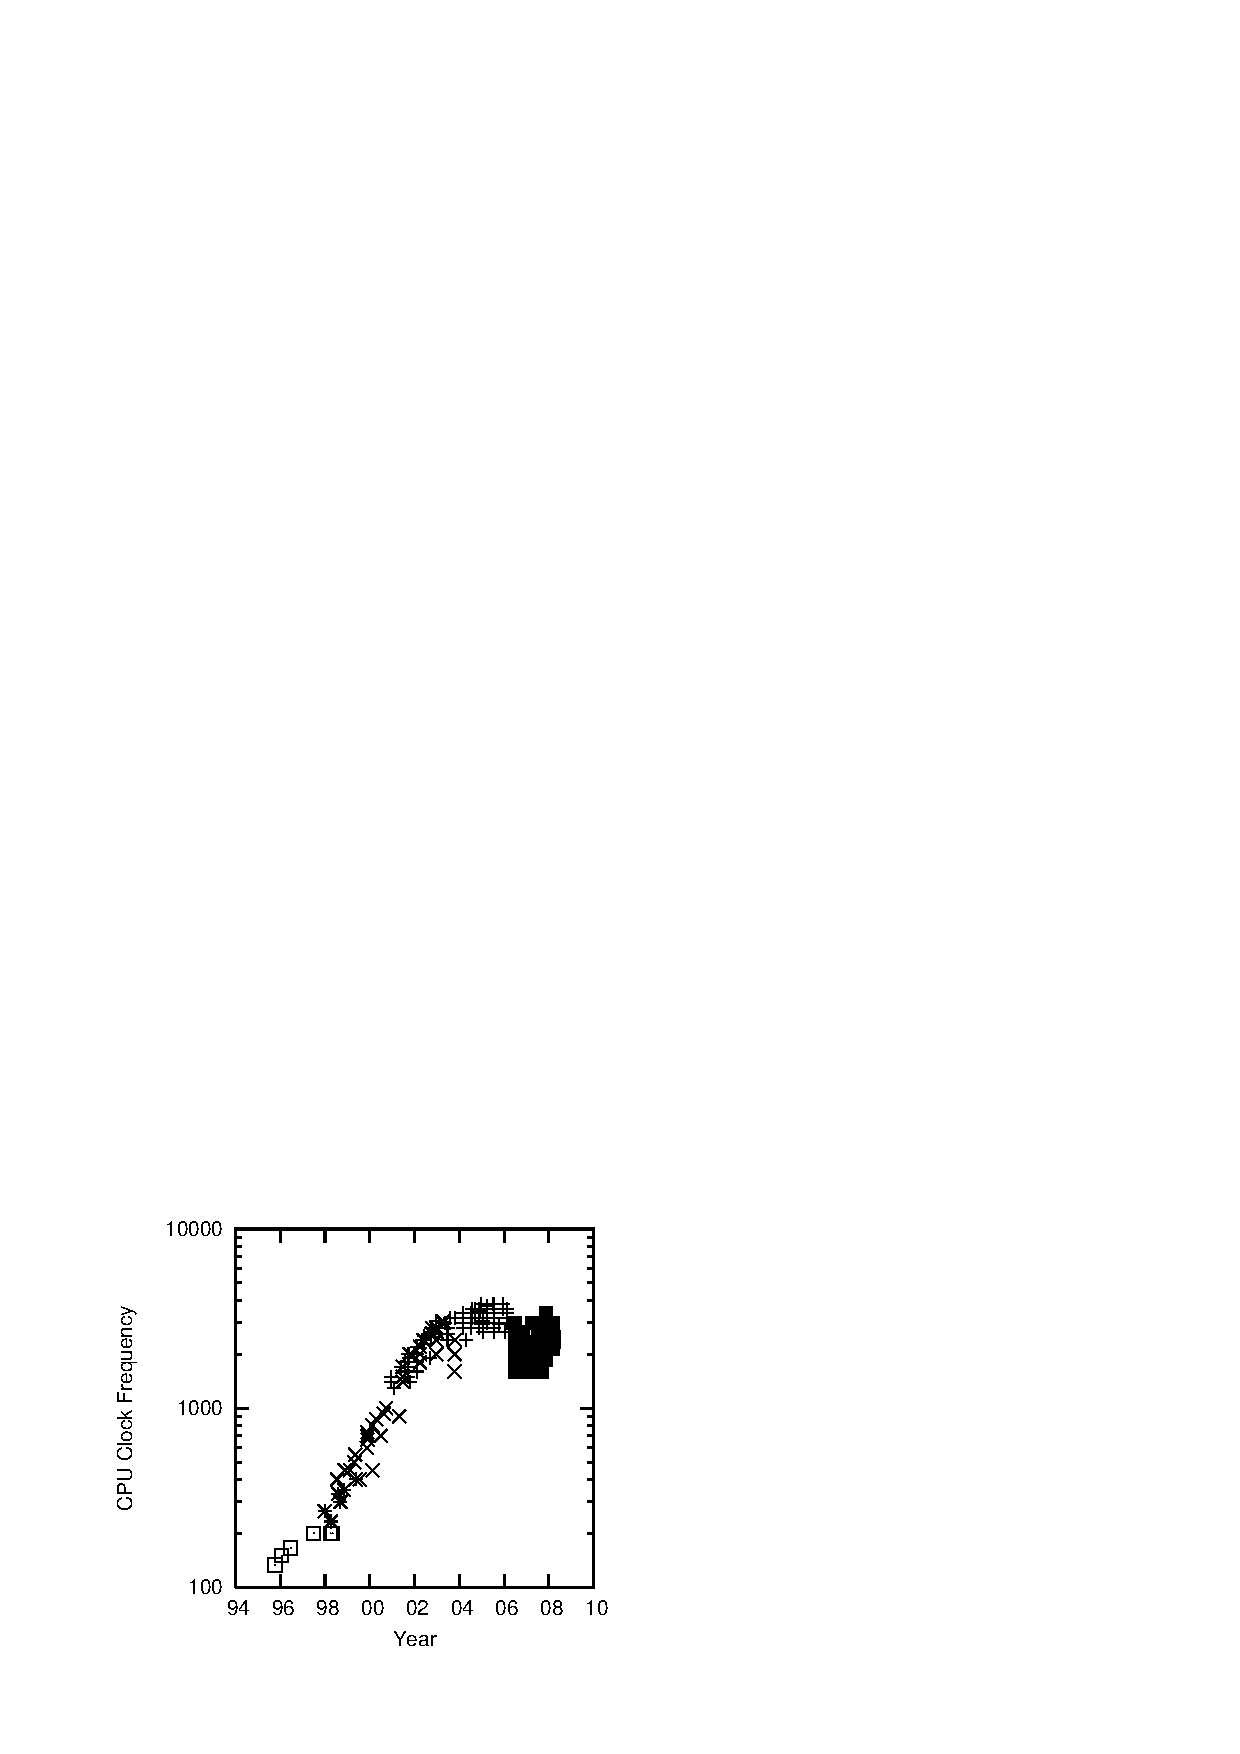
\includegraphics{SMPdesign/clockfreq}}
\end{center}
\caption{Clock-Frequency Trend for Intel CPUs}
\label{fig:intro:Clock-Frequency Trend for Intel CPUs}
\end{figure}

Even so, the first goal is performance rather than scalability,
especially given that the easiest way to attain linear scalability
is to reduce the performance of each CPU~\cite{LinusTorvalds2001a}.
Given a four-CPU system, which would you prefer?
A program that provides 100 transactions per second on a single CPU,
but does not scale at all?
Or a program that provides 10 transactions per second on a single CPU,
but scales perfectly?
The first program seems like a better bet, though the answer might
change if you happened to be one of the lucky few with access to a
32-CPU system.

Therefore, correctness first, performance second,
and scalability only as needed to
attain the required performance on whatever hardware your program
is to run on.

\section{Alternatives to Parallel Programming}
\label{sec:intro:Alternatives to Parallel Programming}

In order to properly consider alternatives to parallel programming,
you must first have thought through what you expect the parallelism
to do for you.
As seen in Section~\ref{sec:intro:Parallel Programming Goals},
typical goals include:

\begin{enumerate}
\item	Improve performance.
\item	Learn more about parallel programming.
\item	Have fun solving a parallel-programming problem.
\end{enumerate}

@@@ Adjust based on HOTPAR submission @@@

Although most developers might be most concerned with the first goal,
one advantage of the other goals is that they relieve you of the need
to justify using parallelism.
The remainder of this section is concerned only performance improvement.

It is important to keep in mind that parallelism is but one way to
improve performance.
Other well-known approaches include the following, in roughly increasing
order of difficulty:

\begin{enumerate}
\item	Run multiple instances of a sequential application.
\item	Construct the application to make use of existing parallel software.
\item	Apply performance optimization to the serial application.
\end{enumerate}

\subsection{Multiple Instances of a Sequential Application}
\label{sec:intro:Multiple Instances of a Sequential Application}

Running multiple instances of a sequential application can allow you
to do parallel programming without actually doing parallel programming.
There are a large number of ways to approach this, depending on the
structure of the application.

If your program is analyzing a large number of different scenarios,
or is analyzing a large number of independent data sets, one easy
and effective approach is to create a single sequential program that
carries out a single analysis, then use any of a number of scripting
enviroments (for example the \url{bash} shell) to run a number of
instances of this sequential program in parallel.
In some cases, this approach can be easily extended to a cluster of
machines.

This approach may seem like cheating, and in fact some denigrate such
programs ``embarrassingly parallel''.
And in fact, this approach does have some potential disadvantages,
including increased memory consumption, waste of CPU cycles recomputing
common intermediate results, and increased copying of data.
However, it is often  extremely effective, garnering extreme performance
gains with little or no added effort.

\subsection{Make Use of Existing Parallel Software}
\label{sec:intro:Make Use of Existing Parallel Software}

There is no longer any shortage of parallel software environments that
can present a single-threaded programming environment,
including relational
databases, web-application servers, and map-reduce environments.
For example, a common design provides a separate program for each
user, each of which generates SQL that is run against a common
relational database.
The per-user programs are responsible only for the user interface,
wiht hte relational database taking full responsbility for the
difficult issues surrounding parallelism and persistence.

\subsection{Performance Optimization}
\label{sec:intro:Performance Optimization}

Up through the early 2000s, CPU performance was doubling every 18 months.
In such an environment, it is often much more important to create new
functionality than to do careful performance optimization.
Now that Moore's Law is ``only'' increasing transistor density instead
of increasing both transistor density and per-transistor performance,
it might be a good time to rethink the importance of performance
optimization.

After all, performance optimization can reduce power consumption as
well as increasing performance.

Performance analysis of sequential programs is well understood,
and will not be discussed further here.

% intro/hwhabits.tex

\section{Hardware and its Habits}
\label{sec:intro:Hardware and its Habits}

Careless reading of computer-system specification sheets might lead one
to believe that CPU performance is a footrace on a clear track, as
illustrated in Figure~\ref{fig:intro:CPU Performance at its Best},
where the race always goes to the swiftest.

\begin{figure}[htb]
\begin{center}
\resizebox{3in}{!}{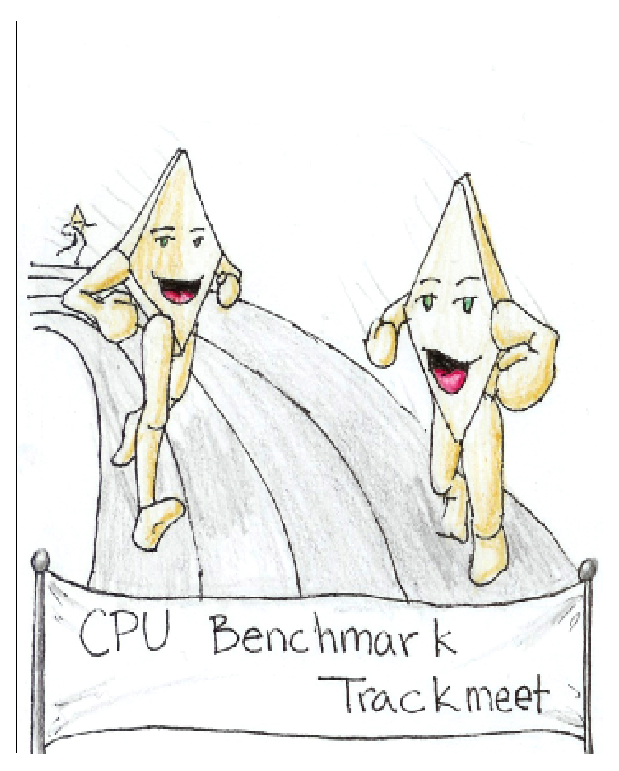
\includegraphics{cartoons/trackmeet}}
\end{center}
\caption{CPU Performance at its Best}
\label{fig:intro:CPU Performance at its Best}
\end{figure}

Although there are a few CPU-bound benchmarks that approach the ideal
shown in Figure~\ref{fig:intro:CPU Performance at its Best},
the typical program more closely resembles an obstacle course than
a race track.
This is because the internal architecture of CPUs has changed dramatically
over the past few decades, courtesy of Moore's Law.
In the early 1980s, the typical microprocessor fetched an instruction,
decoded it, and executed it, typically taking \emph{at least} three
clock cycles to complete one instruction before proceeding to the next.
In contrast, the CPU of the late 1990s and early 2000s will be executing
many instructions simultaneously, using a deep ``pipeline'' to control
the flow of instructions internally to the CPU, this difference being
illustrated by Figure~\ref{fig:intro:CPUs Old and New}.

\begin{figure}[htb]
\begin{center}
\resizebox{3in}{!}{
\includegraphics{cartoons/whippersnapper}}
\end{center}
\caption{CPUs Old and New}
\label{fig:intro:CPUs Old and New}
\end{figure}

\emph{@@@ check up on better .eps for figure.  Also insert block diagram
of CPU.}

Achieving full performance with a CPU having a long pipeline requires
highly predictable control flow through the program.
Suitable control flow can be provided by a program that executes primarily
in tight loops, for example, programs doing arithmetic on large matrices
or vectors.
The CPU can then correctly predict that the branch at the end of the loop
will be taken in almost all cases.
In such programs, the pipeline can be kept full and the CPU can execute
at full speed.

If, on the other hand, the program has many loops with small loop counts,
or if the program is object oriented with many virtual objects that
can reference many different real objects, all with different implementations
for frequently invoked member functions, then it is difficult or even
impossible for the CPU to predict where a given branch might lead.
The CPU must then either stall waiting for execution to proceed far enough
to know for certain where the branch will lead, or guess --- and, in
face of programs with unpredictable control flow, frequently guess wrong.
In either case, the pipeline will empty and have to be refilled, leading
to stalls that can drastically reduce performance,
as fancifully depicted in Figure~\ref{fig:intro:CPU Meets a Pipeline Flush}.

\begin{figure}[htb]
\begin{center}
\resizebox{3in}{!}{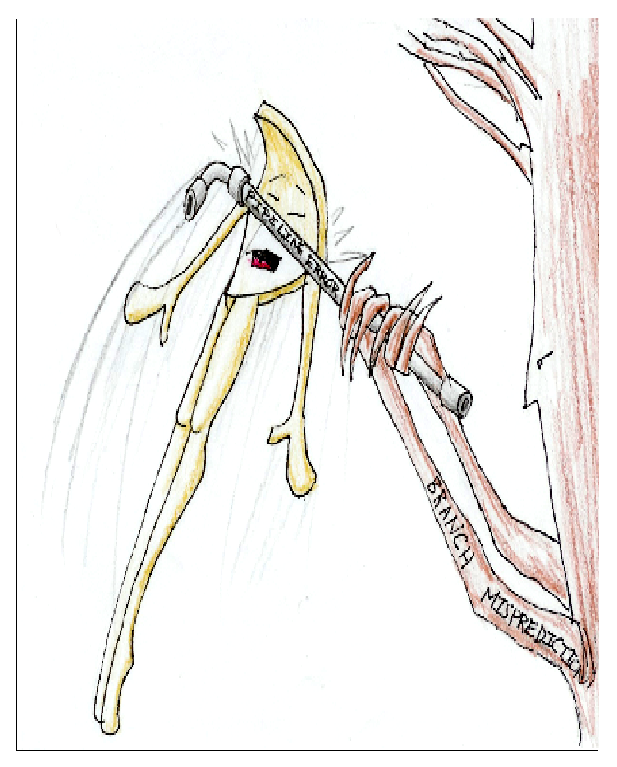
\includegraphics{cartoons/pipeline}}
\end{center}
\caption{CPU Meets a Pipeline Flush}
\label{fig:intro:CPU Meets a Pipeline Flush}
\end{figure}

Unfortunately, pipeline flushes are not the only hazards in the obstacle
course that modern CPUs must run.
In the 1980s, it often took less time for a microprocessor to load a value
from memory than it did to execute an instruction.
In 2006, a microprocessor might be capable of executing hundreds or even
thousands of instructions in the time required to access memory.
This disparity is due to the fact that Moore's Law has increased CPU
performance at a much greater rate than it has increased memory
performance, in part due to the rate at which memory sizes have
grown.\footnote{
	A typical 1980 computer might have 64KB (yes, kilobytes,
	not megabytes, let along gigabytes) of main memory.
	In 2006, CPU designers really can construct a 64KB memory
	with single-cycle access.
	And in fact they do, but it is now called a ``cache''.}

Although the large caches found on modern microprocessors can do quite
a bit to combat memory-access latencies,
just as keeping pipelines full requires highly predictable control flow,
these caches require highly predictable data-access patterns to
successfully hide memory latencies.
Unfortunately, common operations, such as traversing a linked list,
have extremely unpredictable memory-access patterns --- after all,
if the pattern was predictable, us software types would not bother
with the pointers, right?

Therefore, as shown in
Figure~\ref{fig:intro:CPU Meets a Memory Reference},
memory references are often severe obstacles for modern CPUs.

\begin{figure}[htb]
\begin{center}
\resizebox{3in}{!}{
\includegraphics{cartoons/ref}}
\end{center}
\caption{CPU Meets a Memory Reference}
\label{fig:intro:CPU Meets a Memory Reference}
\end{figure}

Thus far, we have only been considering obstacles that can arise during
a given CPU's execution of single-threaded code.
Multi-threading presents additional obstacles to the CPU.

One such obstacle is atomic operations.
The whole idea of an atomic operation in some sense conflicts with
the piece-at-a-time assembly-line operation of a CPU pipeline.
To hardware designers' credit, modern CPUs use a number of very clever
tricks to make such operations \emph{look} atomic even though they
are in fact being executed piece-at-a-time, but even so, there are
cases where the pipeline must be delayed or even flushed in order to
permit a given atomic operation to complete correctly.

The resulting effect on performance is depicted in
Figure~\ref{fig:intro:CPU Meets an Atomic Operation}.

\begin{figure}[htb]
\begin{center}
\resizebox{3in}{!}{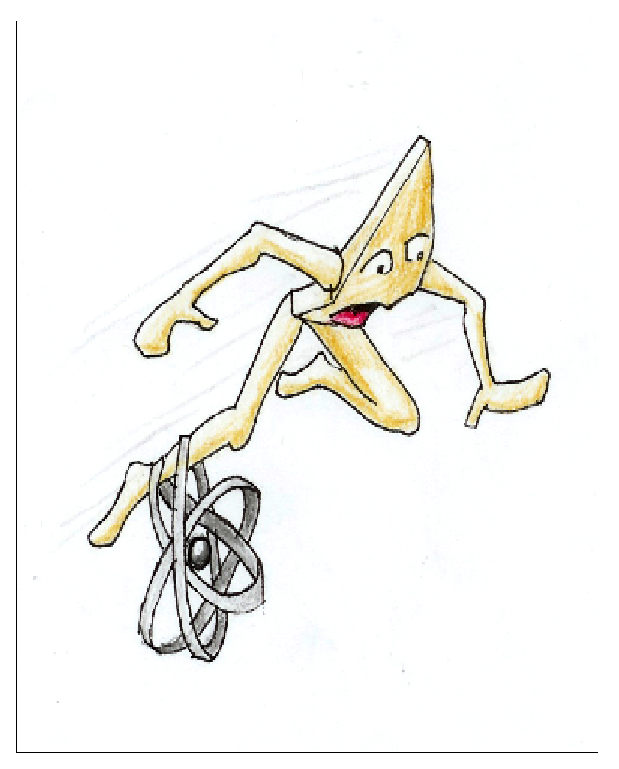
\includegraphics{cartoons/atomic}}
\end{center}
\caption{CPU Meets an Atomic Operation}
\label{fig:intro:CPU Meets an Atomic Operation}
\end{figure}

Another multi-threading obstacle to CPU performance stems from the
need of concurrent algorithms to maintain proper ordering of their
operations, as will be discussed in more detail in
Section~\ref{sec:advsync:Memory Barriers} and
Appendix~\ref{chp:app:whymb:Why Memory Barriers?}.
In the meantime, consider the following simple lock-based critical
section:

\vspace{5pt}
\begin{minipage}[t]{\columnwidth}
\small
\begin{verbatim}
  1 spin_lock(&mylock);
  2 a = a + 1;
  3 spin_unlock(&mylock);
\end{verbatim}
\end{minipage}
\vspace{5pt}

If the CPU were not constrained to execute these statements in the
order shown, the effect would be that the variable ``a'' would be
incremented without the protection of ``mylock'', which would certainly
defeat the purpose of acquiring it.
To prevent such destructive reordering, locking primitives contain
either explicit or implicit memory barriers.
Because the whole purpose of these memory barriers is to prevent reorderings
that the CPU would otherwise undertake in order to increase performance,
memory barriers almost always reduce performance, as depicted in
Figure~\ref{fig:intro:CPU Meets a Memory Barrier}.

\begin{figure}[htb]
\begin{center}
\resizebox{3in}{!}{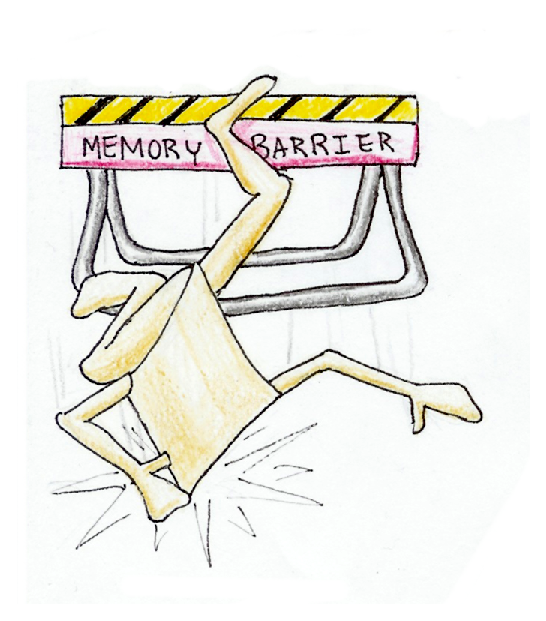
\includegraphics{cartoons/barrier}}
\end{center}
\caption{CPU Meets a Memory Barrier}
\label{fig:intro:CPU Meets a Memory Barrier}
\end{figure}

The final multi-threading obstacle to CPU performance is the ``cache miss''.
As noted earlier, modern CPUs sport large caches in order to reduce the
performance penalty that would otherwise be incurred due to slow memory
latencies.
However, these caches are actually counter-productive for variables that
are frequently shared among CPUs.
This is because when a given CPU wishes to modify the variable, it is
most likely the case that some other CPU has modified it recently.
In this case, the variable will be in that other CPU's cache, but not
in this CPU's cache, which will therefore incur an expensive cache miss
(see Section~\ref{sec:app:whymb:Cache Structure} for more detail).
Such cache misses form a major obstacle to CPU performance, as shown
in Figure~\ref{fig:intro:CPU Meets a Cache Miss}.

\begin{figure}[htb]
\begin{center}
\resizebox{3in}{!}{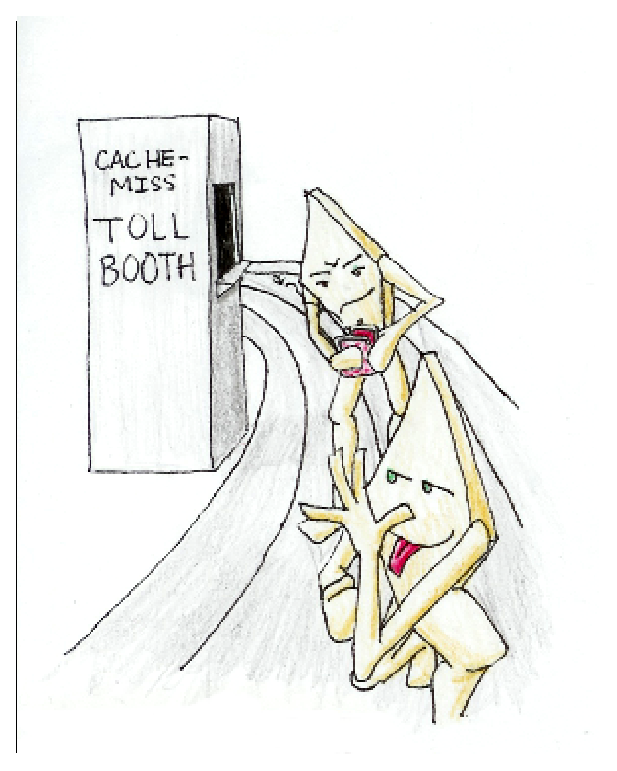
\includegraphics{cartoons/tollbooth}}
\end{center}
\caption{CPU Meets a Cache Miss}
\label{fig:intro:CPU Meets a Cache Miss}
\end{figure}

These obstacles can easily prevent your program from attaining its
potential on today's multi-core and multi-threaded hardware,
in fact, as we will see in Chapter~\ref{cha:SMP Synchronization Design}.
Much of the remainder of this book is dedicated to presenting
design rules, algorithms, and techniques that can help you
overcome these obstacles.


\section{Ease of Use}
\label{sec:intro:Ease of Use}

We are talking about parallel performance and latency,
so why is ease of use important?

Because the easier a performance technique is to use, the more likely
it will be used.
This greater use can outweigh a small performance penalty compared
to an optimal hard-to-use technique.

This book is not a collection of optimal algorithms with tiny areas of
applicability; instead, it is a handbook of widely applicable and heavily
used techniques.
We of course could not resist the urge to include some of our favorites
that have not (yet!) passed the test of time (what author could?), but
we have nonetheless gritted our teeth and banished our darlings to
appendices.
Perhaps in time, some of them will see enough use that we can promote
them into the main body of the text.

\section{Guide to This Book}
\label{sec:intro:Guide to This Book}

\emph{@@@ More here.  Sections.  Layered Approach.  Appendices.
Quick Quizzes.  Glossary.  Bibliography.}

\subsection{Quick Quizzes}

``Quick quizzes'' appear throughout this book.
Some of these quizzes are based on material in which that quick quiz
appears, but others require you to think beyond that section, and,
in some cases, beyond the entire book.
As with most endeavors, what you get out of this book is largely
determined by what you are willing to put into it.
Therefore, readers who invest some time into these quizzes will
find their effort repaid handsomely with increased understanding
of parallel programming.

Answers to the quizzes may be found in
Appendix~\ref{chp:Answers to Quick Quizzes} starting on
page~\pageref{chp:Answers to Quick Quizzes}.

\emph{@@@ Need some quick quizzes...}
